\epigraph{The following chapter was written by the MADRID Team }{\textit{iGEM Madrid\_UCM 2021}}
\section{What is Metabolic Engineering}
Metabolic Engineering (ME) consists in the directed modification and regulation of an organism' metabolic pathways for metabolite over production or the improvement of certain cellular features. Either native pathway engineering, introduction of heterologous pathways or the design of synthetic pathways for converting microorganisms into microbial cell factories can be considered Metabolic Engineering applications. \\ \\
The field of Metabolic Engineering is highly interdisciplinary being closely related with synthetic biology. Metabolic engineering is a complex task which requires the elucidation of existing or novel metabolic pathways, their manipulation and regulation by gene edition techniques as well as efficient probing systems for the implemented metabolic pathways. Then, the application of appropriate methods from molecular biology, along with techniques from engineering  such as modeling and data analysis are a key feature of metabolic engineering. \\ \\
Recently Metabolic Engineering field is evolving towards a systems  biology approach, leading to outstanding advances in strain engineering. Systems Metabolic Engineering aims to speed up the pathway prototyping process and its scale up to industrial processes. In fact, Metabolic Engineering is currently evolving into a novel manufacturing technology where either computational and mathematical analysis are being combined with experimental approaches for rational engineering of microorganisms. Currently, these tools are fueling the development of a new area, where metabolic engineering principles can be even applied in-vitro, where metabolic pathways occurs and regulate completely outside of any organism \parencite{Wei2020}.
\\ \\
\section{Key Notions in Metabolic Engineering}
It is common to observe how allegedly well-designed heterologous pathways experience low yields when implemented into a different organism. There are several reasons for this to happen. Adequate regulation of the pathway is either crucial and a challenging task, which vastly depends on the chassis organism and the availability of well characterized genetic elements. \\ \\
However, the first step for metabolic engineering is to elucidate how a pathway should be regulated, and despite Metabolic Engineering can be a really complex work, there exists several rules of thumb that should be considered into any metabolic engineering design. Within this section you will find some of this basic principles that can be applied for pathway optimization and consequently, increasing the productivity of a certain metabolite.
\subsection{Carbon Flux}
Carbon Flux is they cornerstone of Metabolic Engineering. This concept refers to the way carbon is routed towards the more or less intrincated pathway network which comprises an organism metabolism. Carbon Flux refers to the amount of carbon atoms that are routed from the carbon source/s of an organism towards certain metabolic pathways. Depending on the organism and environmental conditions carbon can be partitioned via many different pathways. \\ \\
Essentially carbon flux consists on a concept that allows to weight the importance of certain reactions within a pathway, considering the amount of carbon which is being converted in the organism via that specific reaction/s.  The higher carbon flux is towards certain pathway, higher production of metabolites related from that pathway could be achieved. \\ \\
Carbon Flux concept is crucial since it allows the visualization of an organism metabolism in a very simple perspective. From this perspective, metabolism can be considered as a pipe network, where there are \textbf{carbon sources} where carbon uptake from outer media occurs, and there are \textbf{carbon sinks} where the acquired carbon escapes the metabolism and virtually stops experiencing transformations. \textbf{Carbon sources} are generated by the first \textbf{carbon assimilation reactions} belonging to catabolism, while \textbf{anabolic reactions} leading to the formation of biomass or metabolites that eventually will be secreted creates \textbf{carbon sinks}. \\ \\
Most of metabolic reactions are reversible, this implies that if a carbon sink is close to a pathway, it will “attract“ carbon flux towards its direction, since the final product of the reaction is being “dragged“ displacing the equilibrium towards the final products. Then an useful strategy for re-routing carbon is to create carbon sinks capable of pulling carbon out from the central metabolism towards the desired reactions. \\ \\
Likewise, carbon flux can provide an idea of which pathway can be more optimally implemented within a certain organism just attending to which set of reactions naturally posses a higher carbon flux. Those pathways which has higher carbon flux will provide a more abundant carbon supply for heterologous pathways feeding on them.
\subsection{Metabolite Availability}
Another crucial aspect to consider is the existence of \textbf{key metabolites} and how available they are. Taking into account the former concept of carbon flux, there exists certain metabolites which are central nodes of several pathways. \\ \\
When designing or implementing a pathway within an organism, it is essential to consider which are going to be the native metabolites to be converted into the desired final product. The most abundant a metabolite is, the easier will be for an alternative pathway to efficiently drag carbon via the desired reactions towards the carbon sink that is the final product. \\ \\
Depending on the chassis organism and its metabolic state, certain metabolites would be more abundant than others. Then selecting those metabolites with higher abundance will result in higher productivities in the end of the pathway. \\ \\
As an example, metabolomic analysis has show that certain cyanobacteria such as \textit{Synechocystis sp.} PCC6803 have an acetyl-CoA availability ten times higher during normal growth conditions compared to \textit{Synechococcus sp.} PCC7002. This “baseline concentration“ of a certain metabolites during normal cell growth is defined as “metabolite pool“. \\ \\
Then another strategy to increase the productivity of a certain pathway is not only to start from a central metabolite which is already highly available within the chassis, but also to implement additional reactions in the metabolic design that increase the conversion of other metabolites towards this “key metabolite“.
\subsection{Branching and Competitiveness in Pathway Networks}
Metabolic pathways often do not take place on a linear fashion, but they rely on several interconnections. When implementing a pathway it is crucial to consider all the already existing pathways within the cell and how can they actually drag or supply carbon to the target pathway. \\ \\
Bothe the final and the intermediate subproducts can be potentially transformed via certain pathway already present within the organism. Therefore a key aspect to consider is the existence of competing pathways, capable of dragging carbon from the desired pathway re-routing it back to other native metabolic functions.
\begin{itemize}
    \item[] An \textbf{example} of this is the ability to synthetize energy storage compounds such as Polyhidroxyalkanoates (PHAs) or Polyhydroxybutyrate (PHBs). Certain bacteria express PHA/PHB synthases, capable of synthetizing PHAs or PHBs from acetyl-CoA derived metabolites. Each PHA synthase converts certain acetyl-CoA derived metabolite (Acetyl-CoA, Acetoacetyl-CoA, R-3-OH-butyryl-CoA, 3-OH-acyl-CoA etc...) into another key metabolite required for the PHA/PHB synthesis pathway.
 
    \item[] When implementing  a pathway which starts from acetyl-CoA as key metabolite, or some of its steps involves the formation of this acetyl-CoA metabolites, considering if the chassis organism is capable of synthetizing PHAs/PHBs or not could be crucial. In PHAs/PHBs synthetizing organisms, the overproduction of some of this intermediate metabolites via the introduced pathway could trigger the synthesis of PHAs/PHBs, reducing the pathway yield or even completely numbing  the formation of the final product. Then, a knock out of this PHAs/PHBs synthase genes will be desirable to enhance pathway productivity. In the other hand, if the chassis organism is not a natural producer of PHAs/PHBs, the pathway could be implemented without further problems, and the intermediate metabolites will mainly be directly channelized towards the final product.
\end{itemize}
Most of this competing pathways are usually found in the early stages of a pathway, where a certain key metabolite is converted into the intermediate precursors of the final product. Key metabolites usually act as a branching point for carbon flux. When possible, usually down-regulating or knocking-down non-essential pathways feeding on the key metabolite is a good strategy for increasing the carbon flux towards the desired pathway.
\subsection{Metabolic Burden and Metabolite Toxicity}
Eventually, one crucial aspect when engineering the metabolism of an organism is the potential toxicity that the introduction of genetic modifications can produce. This toxicity can mainly develop via two different reasons: excessive metabolic burden of the pathway or inherit toxicity of the final product or intermediate metabolites.

\subsubsection{Metabolic Burden}
Most of the pathways start from a very few key metabolites. This leads to a situation where it is common to observe how artificial metabolic pathways suffer from low productivity because carbon is usually preferentially routed towards the native pathways. A common strategy to overcome this issue is to up-regulate the expression of the foreign pathway (codon optimization, use of strong regulatory elements etc). However, the usage of too strong promoters or RBS can lead to impaired cell growth or even cell death. When the expression of a pathway is so high that it comprise even the basic metabolic functions, the metabolic burden of that pathway is high. \\ \\
Metabolic burden can be defined the proportion of the resources of a host cell that are used to operate the artificially introduced or modified pathways  within a host cell. Cell resources can be either energy (ATP and cofactors) or carbon molecules used as building blocks. Consequently, when implementing a pathway in a specific chassis organism, it is crucial to consider what would be the metabolic burden that the pathway and its regulation will impose to the organism.
 
\subsubsection{Metabolite Toxicity}
 
Likewise, some metabolites are toxic to the cells. When a pathway is overexpressed and huge amounts of certain compounds start accumulating in the cell, the toxic effects of the metabolites start becoming stronger till the cells eventually die. Depending on the biochemical nature of the synthetized compounds, toxicity may arise from many different mechanisms. However, in any of this cases, the implementation of supporting genetic modifications, able to relieve the cells from the toxicity of the product, is a common strategy to increase the pathway productivity.
\begin{itemize}
    \item[] An \textbf{example} of this is the production of biofuels using microorganisms. Most of biofuels are lipophilic or at least the molecule harbors a lipophilic region. This feature of the final product and some of its intermedium metabolites generate cell toxicity via the interaction with cell membranes
    \item[]It is common to observe that microorganisms modified only for the overproduction of free fatty acids, fatty acids methyl esters, short to medium chain alcohols, alkanes or isoprenoids (all of them promising biofuel candidates) usually suffer from impaired cell growth and moderate yields. When cultures grow for long periods of time, accumulation of desired products starts to plateau as a consequence of the toxicity of the product.
    \item[]Among the common strategies to overcome this problems are the selection of robust chassis organisms with native mechanisms for solvent tolerance like yeasts or the implementation of secretion mechanisms for pumping out the toxic products from the interior of the cells.
\end{itemize}

\subsection{Pathway Design}
\textit{Metabolic Engineering} relies either in the optimization of already existing pathways and its adaptation to other heterologous chassis and the design and implementation of \textit{de novo} artificially designed pathways. Currently the field of \textit{metabolic engineering} is evolving fast towards the computer-aided design of pathways at the genomic level, taking into account all the potential interactions between the already-existing pathways of a chassis organism, and the possible reaction schemes that could be implemented to achieve specific goals. \\ \\
Despite the aim of this chapter is not to provide a deep insight within how to design metabolic pathways but establish the guidelines for smart pathway design, it is important to remark the existence of several tools for pathway design and optimization. To know more about, Otero-Muras \& Carbonell covered extensively this topics in the review article cited in the references.
\section{Phototrophs Metabolic Engineering}
An heterotrophic organism such as \textit{S. cerevisiae} feeding on sugars will route most of the carbon towards the glycolysis pathway and after that carbon flux will start branching in different routes. Part of it will be derived towards the energy metabolism, becoming CO2 or ethanol, while other part of the carbon flux will be redirected to anabolism becoming part of the cell constituents or secondary metabolites used for defense or communication. In short, heterotrophic metabolism uses organic compounds as both carbon and energy sources. \\ \\
On the other hand a phototrophic organism route most of the carbon towards the Calvin–Benson–Bassham (CBB) cycle or similar carbon fixation pathways. CO2 and the solubilized HCO3- are used as the main carbon sources, while the energy comes from the environmental light. In a phototrophic organism, energy is harvested during the light step of the photosynthesis, while carbon is captured during the dark phase of the photosynthetic process. A deep comprehension of this aspects is essential to truly understand phototrophic metabolism.
\subsection{Phototrophic Organisms and Phototrophic Metabolism}
Phototrophic metabolism widely differs from the conventional heterotrophic systems. Despite the huge differences among the different phototrophic metabolism there exists certain features that phototrophic organism share and makes them different from other standard chassis in synthetic biology. \\ \\
In addition, it is important to remark that the availability of well characterized regulatory elements, standardized protocols, measurement methods and metabolic models for phototrophs still long way behind all the tools available for heterotrophs. \\ \\
One key aspect is the \textbf{cofactor abundance (NADPH / NADH ratio)}. In heterotrophs NADH is the main cofactor, produced during the energy metabolism and mainly used for catabolic pathways. Meanwhile NADPH is mainly employed for anabolism and obtained via the interconversion of formerly generated reducing power. In phototrophs NADPH is the principal cofactor generated during photosynthesis and the NADPH pool is much more abundant than the NADH one. This is a common characteristic of phototrophs and one of the reasons why heterologous pathways coming from heterotrophs usually display poor yields when cloned into phototrophic chassis. \\ \\
Another important aspects and differences between the principal phototrophic chassis are detailed in the table below:

\begin{figure}[!htpb]
    \centering
    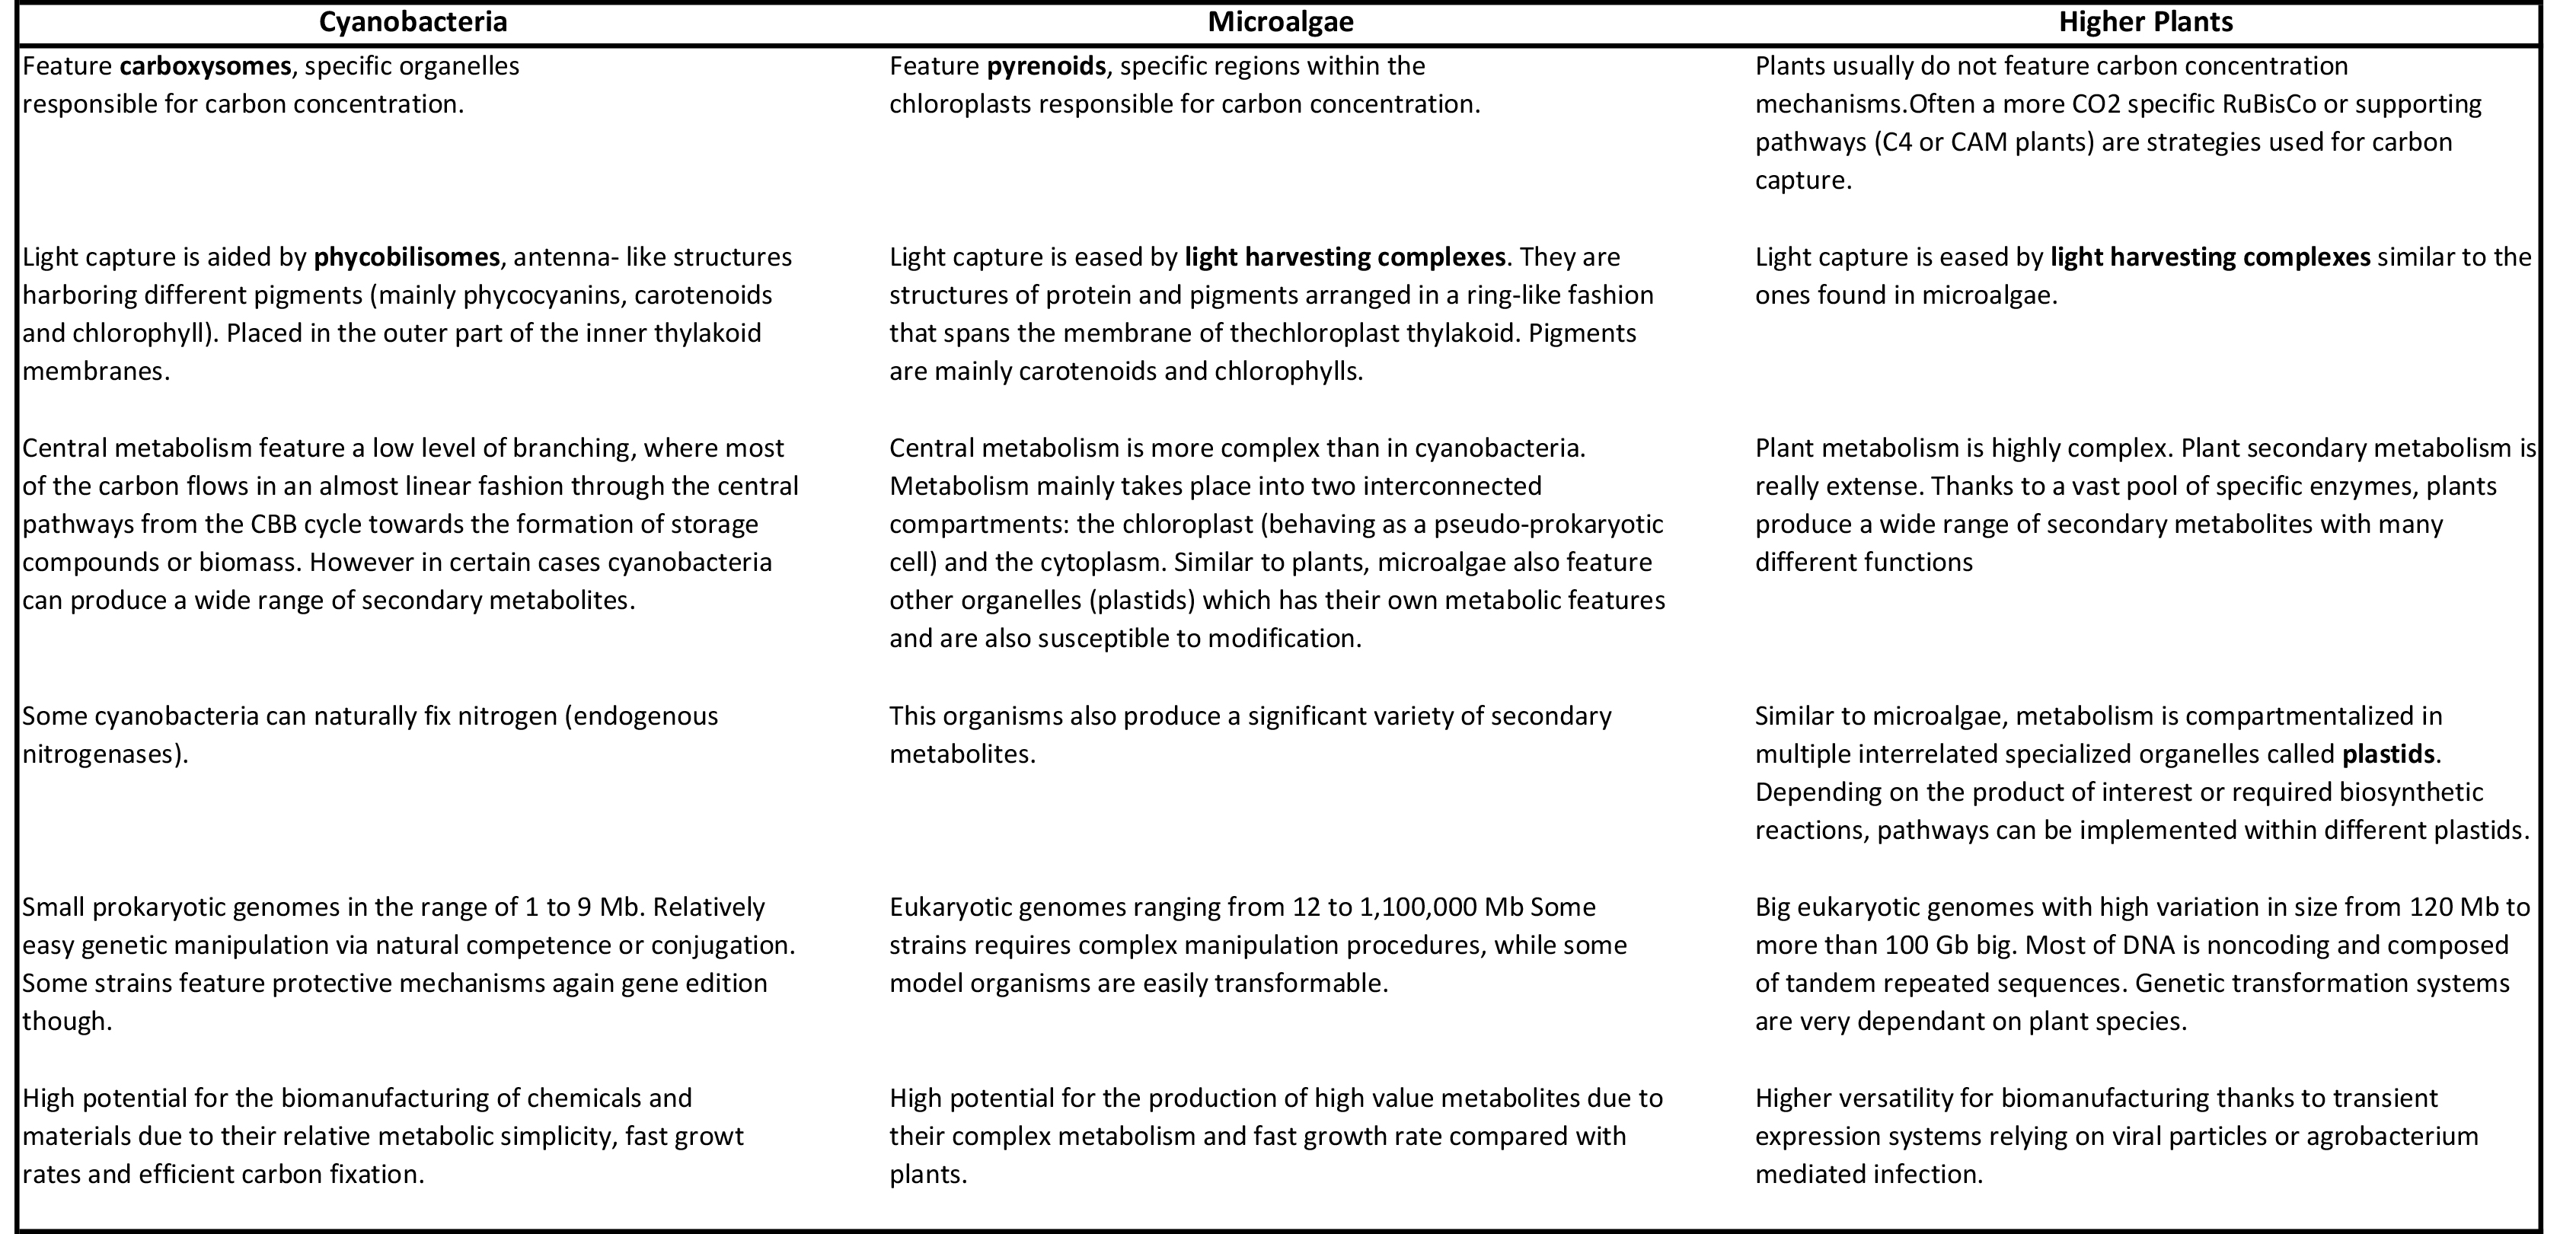
\includegraphics[angle=-90, scale=0.2]{images/chap7/table_met_eng.jpg}
    \label{fig:chp7landscapetable}
\end{figure}
\FloatBarrier
\noindent
Briefly, it is important to consider that phototrophic metabolism is different from heterotrophic organism. Thus metabolic engineering of phototrophs will require specific considerations and design rules that could differ to the ones applied in heterotrophs. \\ \\
All the formerly introduced concepts still applying for metabolic engineering of phototrophs. However, there are some key aspects that must be taken into account to efficiently engineer the metabolism of phototrophic organisms and harness their full potential as photosynthetic bio-factories. \\ \\
The subsequent sections will provide a brief insight within the strategies that can be implemented within a phototrophic chassis in order to enhance the productivity of metabolic pathways.
\subsection{Strategies to Enhance Carbon Fixation}
While heterotrophs rely on the availability of different carbon sources, phototrophs depens on an unique substrate: Carbon Dioxide (CO2). CO2 or its solubilized form (HCO3-) is the source of all phototrophic metabolism. Then enhancing the ability of an organism to fix carbon and pump it through its metabolism is the first step to optimize the productivity of any pathway. The highest input carbon flux the metabolic network has, the higher availability of carbon will be for any reaction. This way, several strategies can be implemented in order to maximize the carbon fixation.
 \begin{itemize}
     \item[] \textbf{RuBisCO engineering}. Ribulose-1,5-bisphosphate carboxylase-oxygenase or RuBisCO is the enzyme responsible for carbon fixation in almost any photoautotrophic organism. However RuBisCO is rather inefficient and high amounts of the enzyme are produced in order to allow the cells fix enough carbon for their survival. Likewise, RuBisCo can catalyze the oxidation of Ribulose-1,5-bisphosphate, producing 2-phosphoglycolate, a toxic metabolite that must be recycled via the photorespiratory metabolism, loosing carbon and spending energy.
     \item[] To avoid the photorespiration drawbacks each organism has evolved their own version of RuBisCO variants. RuBisCO in cyanobacteria is highly active and efficiently catalyzes carbon fixation. However its selectivity towards CO2 is poor. On the other hand, plant RuBisCO is less active than the cyanobacterial counterparts (even 3 times less active), but the selectivity towards CO2 is up to twice higher.
    \item[] Depending on the chassis organism and desired conditions for the organism development, the introduction of heterologous or engineered RuBisCO variants can be a strategy for improved carbon fixation. However, despite RuBisCO engineering has been attempted several occasions, most of the published bibliography demonstrates that only moderate improvements can be achieved, and most of the time selectivity should be compromised in favour of activity or vice-versa.
 
\item[] \textbf{Reducing carbon loss}.  Photorespiration as well as other pathways reduces the overall capacity of an organism to assimilate carbon from CO2. Certain metabolic pathways can release carbon molecules as CO2, HCO3-, but photorespiration still being the main process responsible for carbon and energy loss. Photorespiration can lead to a reduction of up to 30\% of the overall metabolic capacity of the organism. Some recent studies has shown the potential role of RuBisCO oxygenase activity in nitrite assimilation and protein synthesis, however photorespiration still being a metabolism branch which can be highly optimized.
    \item[] Several synthetic pathways has been designed in order to reduce the energy expense and carbon losses generated via the photorespiration. Most of this schemes rely on the reconversion of intermediate photorespiration metabolites into the central carbon fixation pathway metabolites.
    \item[] In addition, some artificial pathways has been designed in order to enhance carbon fixation via optimized carbon fixation reactions that could exceed the efficiency of natural pathways such as the CBB cycle.
\item[] \textbf{Carbon Concentration Mechanisms}. Many phototrophs feature specializations that allows them to fix carbon more efficiently. The most common strategy is to increase the CO2 concentration in the cellular compartments where RuBisCO is expressed, this strategies are defined as Carbon Concentration Mechanisms (CCM).
    \item[] An example of CCMs are carboxysomes. Carboxysomes are a cyanobacteria-specific CCM in order to cope with the lower selectivity of their RuBisCO variants. Initially the cell firstly generates a high intracellular bicarbonate (HCO3−) pool through action of membrane inorganic carbon transporters and CO2-converting complexes. This bicarbonate will subsequently be reconverted into CO2 in the carboxysomes to enhance carbon fixation.
    \item[] Carboxysomes are pseudo-organelles composed of polyhedral protein forming a capsid. This capsid is thighly assembled, generating an environment where gaseous CO2 diffusion is impeded. Within the capsid structure carbonic anhydrase (which converts the soluble HCO3- into CO2) , and RuBisCO  are embedded. This way, within the carboxysome CO2 concentration is between 10 to 100 times higher than the external concentration, increasing RuBisCO activity and promoting the selectivity of the catalysis towards carboxylation.
Microalgae feature their own CCMs, while only certain plants have evolved specific adaptations such as the C4 or CAM plants specific carbon concentration mechanisms. In general, every CCM consist on the compartmentalization of carbon fixation reactions in specific environments, where RuBisCO is exposed to higher concentrations of CO2 and lower O2 concentrations, promoting carbon fixation. \\ \\
Either natural or artificial CCMs can be implemented within a chassis in order to improve their carbon fixation efficiency. As an example, some authors have demonstrated an improvement on plant growth rates when cyanobacterial carboxysomes were expressed in the plant chloroplast.
\end{itemize}

\subsection{Strategies to Enhance Light Harvesting}
All phototrophic organisms rely on their ability to convert light into energy, then, the optimization of the light capture phase of the photosynthetic process will allow to increase the efficiency and performance of engineered photosynthetic organisms. To reach that aim, it is necessary to clearly consider the aim of the improvement, in a way that the modification allows for a better performance of the organisms or engineered system in the conditions of the real application. Depending on the conditions of the final application there can be two main possibilities. Either the optimization for high-performance photosynthesis in controlled or favorable environments , or the optimization for high-resistant organisms, able to perform photosynthesis in harsh conditions. \\ \\
The overall photosynthetic performance currently balances between 0.1-1\% in, in some special cases around 2-4\% for plants. Other phototrophs such as cyanobacteria or microalgae can feature slightly higher efficiencies, however the maximum theoretical value is around 10-13\%. The observed relative inefficiency of photosynthesis is derived mainly from the high number of steps involved in photosynthetic process and numerous energy sinks found across the photosynthetic process. In general, there exist three main factors limiting the photosynthetic process: Light, Temperature and CO2 concentration. Controlling either carbon concentration (as explained formerly) or temperature tolerance (enhancing strains robustness and pathway flexibility) can also improve the metabolic performance. However during this section the focus will be made in enhancing light capture.\\ \\
Considering all the aspects involved in the light-phase, multiple bottlenecks for the photosynthetic process can be found. Those critical steps can be used as key points for enhancing light capture performance.
 
\subsubsection{Light Capture Engineering}
First stages of light capture are physical processes involving fast electron transfer reactions with a quantum background. All phototrophs feature specific structures dedicated to light capture, either the Antenna Complex of plants and microalgae, or the phycobilisomes in cyanobacteria and red algae. The modification of these light harvesting systems can directly alter the efficiency of light light to energy conversion within the initial stages of photosynthesis.
\begin{itemize}
    \item[]  \textbf{Light harvesting systems modification} Optimizing the configuration of antenna or light harvesting complexes according with a defined purpose can increase the overall performance. \\ \\
    For example, in the case of microorganisms which will be grown in suspension, truncated antennas can help, reducing the shading effects in bioreactor settings and enhancing overall light absorption. On bioreactor setup or systems where multiple cells are superposed, it allows to distribute the light absorption more efficiently along all the system.  This way there are less cells over-exposed to light (photoinhibition) and less cells experiencing shading. So that, a higher light-stress tolerance and smaller light-to-heat dissipation is achieved. On the other hand higher and pigment-enriched antennas can result in harsh low-light conditions or specific applications.
    \item[] \textbf{Expanding absorbance spectra}. The usage of novel light-absorbing pigments or even different pigments in the reaction centers can enlarge the available light, driving to a higher performance. \\ \\
    As an example, some pigments such as the pigment b-phycoerythrin  of cyanobacteria and red algae feature a light-harvesting efficiency of 98\% compared to the 12\% of pigments found in plants. \\ \\
   Likewise, including different pigments capable of absorbing in other wavelengths , different from the ones that typical light harvesting systems possess can enhance the overall performance of the process. Apart from chlorophyll a, b , carotenoids and similar pigments, there are other pigments that can be used to expand the photosynthetic usable light range.\\ \\
    As an example, most phototrophs can not use light above 700 nm wavelengths. However, some cyanobacteria like \textit{Acaryochloris marina} own a special chlorophyll, able to capture light even in longer wavelengths. It possesses two different chlorophyll molecules:  chlorophyll-d (photosynthetic active center) and chlorophyll-f (light harvesting pigment). That pigments can harvest light at even 760 nm wavelengths. In that organisms, Photosystem I uses Chl.- f, absorbing at 745 nm and Photosystem II is enriched with chlorophyll-f , absorbing at 727 nm. So that, an enhanced usable light spectrum can push the photosynthetic theoretical efficiency from sunlight at a value near 19\%.
 \end{itemize}
However, it is important to consider that although its modifications enhance photosynthetic performance, and grow rates, the modified organisms tend to loose competitiveness against wild-type ones, which has naturally evolved a favorable phenotype. Then rational engineering of light harvesting should always take into account the final application of the engineered organism or system.
 
\subsubsection{Photoprotection Mechanisms}
 
Phototrophic organisms have evolved to adapt to the changing conditions in temperature, irradiance and even CO2 availability. From all of them, light irradiance is the parameter subjected to higher fluctuations. There exists a complex network of different systems that modulate photosynthetic response attending to different changes in the environment. While useful for organism survival, many of these mechanisms lead to energy losses, reducing the efficiency of light-to-energy conversion.\\ \\
These mechanisms widely vary between the organisms, but as general examples are the cyclic electron transfer pathway usually used to balance the ATP/NADPH ration during photosynthesis or the water-to-water cycle, only ATP but no NADPH is produced. That process involves PSII, Cytochrome b6f and PSI. Thos pathways are usually overexpressed during stress conditions, usually during excess reducing power production or excessive photon irradiation. In that condition they dissipate the excess of energy and reduce the generation of highly reactive species that could damage photosynthetic machinery. \\ \\
Some of the strategies that can be followed to enhance light-to-energy conversion are:
\begin{itemize}
    \item[] \textbf{Elimination of energy sinks}. Optimizing the metabolic pathways regulation to avoid entering in cyclic electron flows where the excess of light is not used as energy.
    \item[] \textbf{Relaxing photoprotection systems}. Accelerating the relaxation of energy dissipation an non-photochemical quenching processes can also enhance the overall efficiency.
\end{itemize} 
In general terms, photoprotective mechanisms can widely differ among the different phototrophic chassis. However, altering their pathways in order to reduce the energy sink sizes and modifying the feedback regulation mechanisms to be faster and more precise can also increase overall process efficiency via an useful redirection of the energy surplus produced during intense irradiation periods.  However, these modifications have to be carefully made, to avoid damage in the system, especially when the final usage conditions of the engineered organisms can not be controlled.
 
\subsection{Other Guidelines for Phototrophs Metabolic Engineering}
Eventually, there are some tips and considerations that should be  taken into account when metabolic engineering a phototrophic organism.
\begin{itemize}
\item[] \textbf{NADPH / NADH ration consideration}. When engineering a pathway for a phototrophic organism, certain enzymes would be NADH dependent. In this situation the cellular NADH pool will be crucial for the pathway performance. Avoiding an excessive number of NADH-dependent steps can improve the behaviour of tha pathway. Furthermore the screening for NADPH-dependent enzyme variants with similar activity will be desirable when designing a pathway.
\item[]In the situations where only NADH dependent enzymes feature the desired catalytic function or activity, the implementation of supporting pathways capable of balancing the NADPH / NADH ratio within the organism could be considered. \\ \\
\item[] \textbf{Shorter pathways perform better}. In general, the shorter a pathway is, the more efficient it tends to be. Minimizing the number of reaction steps allows the carbon to flow more efficiently towards the final product, avoiding its loss in competing pathways, or the  reduction in the concentration of the precursor pool into several intermediate metabolites.
\item[] \textbf{Considering the influence of the environment and light cycles}. Most phototrophic organisms feature complex regulatory systems depending on light. As well as other environmental factors, light availability is crucial to determine the metabolic state. Changes in environmental conditions and illumination will produce changes in the metabolism regulation. Among many other aspects, the differential expression of transcription factors can widely alter the central metabolites availability, switch on or off certain native pathways and modify the behaviour of regulatory elements also included within the engineered pathway regulation.
\item[]It is also important to notice that foreign regulatory elements can behave differently within the chassis or even modulate their behavior depending on the cellular state.
\item[] \textbf{Using irreversible reactions as pathway driving-forces}. Most enzymes catalyze reversible reactions, then if a high amount  of a product / intermediate metabolite is produced, the carbon flux across the pathway will be reduced. The introduction of irreversible enzymatic steps (usually addition reactions catalyzed by lyases) , can act as a pathway driving force. Ideally, these irreversible steps should be carefully placed in the critical points of the pathway: in the final conversion step towards the product (avoiding product reconversion) and in the initial pathway steps, where the employed central metabolite could be regenerated.
\item[] \textbf{Codon Usage}. As any other organism, each class of phototrophic organisms will feature a specific codon usage and tRNA availability. Likewise, in cyanobacteria and eukaryotic plasts, it is common to find many open reading frames with alternative start codons such as GTG or TTG. When expressing heterologous genes within phototrophs it is crucial to optimize the codon usage to the classis tRNA availability in order to optimize the transcription process and enhance expression levels.
\end{itemize}
\section*{References}
\parencite{Yadav2018} \parencite{Wuest2011} \parencite{Teng2020} \parencite{Wei2020} \parencite{Tang2011} \parencite{Asplund-Samuelsson2021} \parencite{Jablonsky2016}
\parencite{Otero-Muras2021} \parencite{Zhou2019} \parencite{Shih2016} \parencite{Nielsen2003} \parencite{Wang2017} \parencite{Hanson2016} \parencite{Fang2018} \parencite{Long2018} \parencite{Liang2018} \parencite{Lowe2021} \parencite{South2019} \parencite{Roell2021} \parencite{Xin2014} \parencite{Khurshid2020} \parencite{Basler2016} \parencite{Bloom2018} \parencite{Lea-Smith2016}